\documentclass[a4paper,10pt]{article}
\usepackage[utf8x]{inputenc}
\usepackage{graphicx}
\usepackage{geometry}

\geometry{
body={160mm,230mm},
left=25mm,top=25mm,
headheight=25mm,headsep=7mm,
marginparsep=4mm,
marginparwidth=20mm,
footnotesep=50mm
}

%opening
\title{Software Architectures
Assignment 3: Service Oriented Architectures}
\author{Dehouck Samuel, Delhaye Quentin}

\begin{document}

\maketitle

\section{Introduction}

\section{BPEL Processes}

\subsection{Parallelization}
Before any modification of the process, the different actions done in the main sequence were:
\begin{itemize}
 \item receiveInput: receives input from the requester.
 \item PrepareResponse: prepares the response variable.
 \item AssignSearchRequest: assigns the parameters.
 \item InvokeSearchBooks: invokes the search in the SoftLab library. 
 \item AssignSearchRequest: assigns the parameters.
 \item InvokeSearchForBooks: invokes the search in the National library.
 \item AssignResultSoftLib: assigns the result to the response.
 \item replyOutput: sends the response to the requester.
\end{itemize}

As we can see, the first two actions need to be done sequentially: we need to receive the input first before preparing the response. The same goes for the last two: we need to prepare the response before sending it.
The last two pairs of \textit{Invoke-Assign} are unrelated and their execution can be separated.
In order to parallelize these two couples, we need to use flows. A flow is declared using the tag \texttt{\textless bpel:flow\textgreater}, in which all the declared sequences (using \texttt{\textless bpel:sequence\textgreater})will be executed at the same time.

A graph representing the execution can be found on figure~\ref{fig:graph_seq}

%\vspace{2cm}
 \begin{figure}[h]
	 \centering
 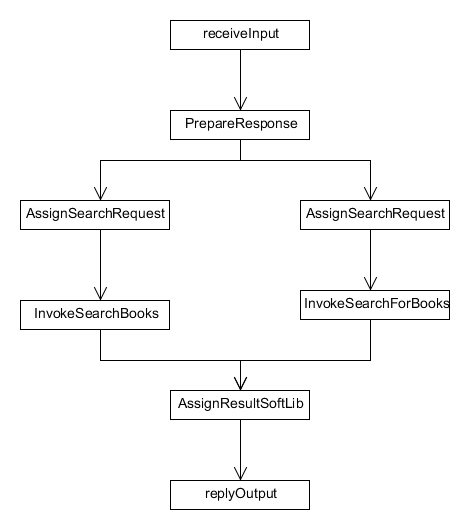
\includegraphics[width=7cm]{diagsequence.png}
 \label{fig:graph_seq}
 \caption{Execution of the BPEL process.}
\end{figure}




\subsection{Data Structure Strategy}
In this table, we describe how books are defined in each library. \\

\begin{center}
\begin{tabular}{|c|c|c|}
\hline
  & National Library & SoftLab Library \\
  \hline
  Author & String & String \\
  \hline
  Date & DateTime & Int \\
  \hline
  ISBN & String & Int \\
  \hline
  Language & String & Language \\
  \hline
  Publisher & String & String \\
  \hline
  Title & String & String \\
  \hline
\end{tabular}
\end{center}
\vspace{0.8cm}

 In order to ease the use of the \textit{LibrarySearch} by additional services, we could normalize the data. There are two ways:
 \begin{itemize}
  \item We could use the types defined by the National Library. But in order to convert the data from the SoftLab Library, we would need to change the year in a full date (day, month and year).
  Some false informations would then be created. The transformation from a \textit{String} to an \textit{Int} would be made without any loss but from a \textit{String} a type \textit{Language}, it would depend on 
  how \textit{Language} is implemented.
  \item We could use the types defined by the SoftLab Library but we would then loose some informations about the date for instance.
 \end{itemize}
 
 As we can see, both choices are valid and the choice would depend on the case.



\section{Integration with Legacy Software}
In order to access the remote web services, we added a new package \texttt{softarch.portal.db.LibrarySearch} containing two classes: \texttt{DatabaseRemote} and \texttt{RegularDatabaseRemote}.
Those are used in the constructor of \texttt{DatabaseFacade} by initializing a regular remote database, no matter what local database configuration has been chosen.

On top of that, the \texttt{findRecords()} method had to be modified.
It now searches in both local and remote databases, and then concatenates the respective results into one single list of \texttt{Book} to return.

The data mapping from \texttt{librarysearch.soft.Book}\footnote{From the client code generated from the \textsc{wsdl} specification.} to \texttt{softarch.portal.data.Book} is done in \texttt{RegularDatabaseRemote.findRecords()} method.
The results from the \textsc{bpel} process are stored in a list of \texttt{Book} of the first type, which is then iterated over and from which each field is extracted and stored in a list of \texttt{Book} of the second type.

The advantage of doing so is that the translation is kept in one place, but adding a new field in the web service book type, or modifying any field would require a modification in this process as well.

\section{Architecture}

\section{Conclusion}

\end{document}
